\documentclass{article}
\usepackage[utf8]{inputenc}
\usepackage[fontset=ubuntu]{ctex}  %中文,编译器选择XeLatex

\title{第四章相机模型与非线性优化作业}
\author{王其超}
\date{February 2021}

\usepackage{natbib}
\usepackage{graphicx}

\begin{document}

\maketitle

\section{Introduction}
我是王其超There is a theory which states that if ever anyone discovers exactly what the Universe is for and why it is here, it will instantly disappear and be replaced by something even more bizarre and inexplicable.
There is another theory which states that this has already happened.

\begin{figure}[h!]
\centering
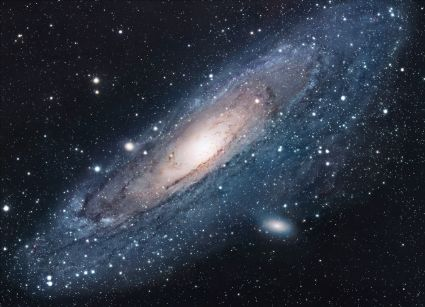
\includegraphics[scale=1.7]{universe}
\caption{The Universe}
\label{fig:universe}
\end{figure}

\section{Conclusion}
``I always thought something was fundamentally wrong with the universe'' \citep{adams1995hitchhiker}

\begin{figure}[h!]
\centering

\includegraphics[scale=0.1]{haha}
\caption{截图}
\label{fig:haha}
\end{figure}

\bibliographystyle{plain}
\bibliography{references}
\end{document}
